\documentclass[xcolor={dvipsnames, svgnames, x11names, table}, 10pt]{beamer}
\usepackage{./assets/preamble}

% \setbeameroption{show notes} % un-comment to see the notes

% \usepackage{pgfpages}
% \pgfpagesuselayout{8 on 1}[a4paper,border shrink=5mm]

\title{Introduzione al corso}
\date{14 settembre 2021}
\institute{%
    \textbf{Obiettivi di apprendimento}:
    \begin{itemize}
        \item Storia recente del \cplusplus;
        \item Esempi di composizione opzionale.
    \end{itemize}%
}

% arara: xelatex: { synctex: no }
% arara: xelatex: { synctex: yes }
% arara: latexmk: { clean: partial }
\begin{document}

\frame{\titlepage}

\begin{frame}{Sommario}
  \setbeamertemplate{section in toc}[sections numbered]
  \tableofcontents%[hideallsubsections]
\end{frame}

\section[Introduzione]{Introduzione}

\begin{frame}[fragile]{\cplusplus e le sue evoluzioni}
\frametitle{Basic Code II - The Frame} % Bookmark info
\framesubtitle{Subtitle} % Bookmark info
    \begin{itemize}[<+- | alert@+>]
        \item \textbf{1979}: Start of work on \enquote{C with Classes} that became \cplusplus; first non-research user;
        \begin{itemize}\footnotesize
            \item \textbf{Language}: classes, constructors/destructors, public/private, simple inheritance, function argument type checking;
            \item \textbf{Library}: tasks (coroutines and simulation support), vector parameterized with macros.
        \end{itemize}
        \item \textbf{1985}: First commercial release of \cplusplus; TC++PL1 [Stroustrup 1985b];
        \begin{itemize}\footnotesize
            \item \textbf{Language}: virtual functions, operator overloading, references, const;
            \item \textbf{Library}: complex arithmetic, stream I/O.
        \end{itemize}
        \item \textbf{1998}: C++98, the first ISO C++ standard [Koenig 1998], TC++PL3 [Stroustrup 1997];
        \begin{itemize}\footnotesize
            \item \textbf{Language}: namespaces, named casts, bool, dynamic\_cast;
            \item \textbf{Library}: the STL (containers and algorithms), string, bitset.
        \end{itemize}
        \framebreak
        \item \textbf{2011}: C++11 [Becker 2011], TC++PL4 [Stroustrup 2013]
        \begin{itemize}\footnotesize
            \item \textbf{Language}: memory model, auto, range-for, constexpr, lambdas, user-defined literals;
            \item \textbf{Library}: threads and locks, future, unique\_ptr, shared\_ptr, array, time and clocks, random numbers, unordered containers (hash tables).
        \end{itemize}
        % \item \textbf{2014}: C++14 [du Toit 2014]
        % \begin{itemize}\footnotesize
        %     \item \textbf{Language}: generic lambdas, local variables in constexpr functions, digit separators;
        %     \item \textbf{Library}: user-defined literals.
        % \end{itemize}
        % \item \textbf{2017}: C++17 [Smith 2017]
        % \begin{itemize}\footnotesize
        %     \item \textbf{Language}: structured bindings, variable templates, template argument deduction from constructors;
        %     \item \textbf{Library}: file system, scoped\_lock, shared\_mutex (reader-writer locks), any, variant, optional, string\_view, parallel algorithms.
        % \end{itemize}
        % \framebreak
        % \item \textbf{2020}: C++20 [Smith 2020]
        % \begin{itemize}\footnotesize
        %     \item \textbf{Language}: concepts, modules, coroutines, three-way comparisons, improved support for compile-time computation;
        %     \item \textbf{Library}: concepts, ranges, dates and time zones, span, formats, improved concurrency and parallelism support.
        % \end{itemize}
    \end{itemize}
    
    % \begin{block}{Modifica librerie vs linguaggio}
    %     Si predilige la modifica delle librerie alla modifica del linguaggio e quindi del compilatore.
    % \end{block}
\end{frame}

% \begin{frame}{Popolarità del \cplusplus}
%     \begin{figure}\centering
%         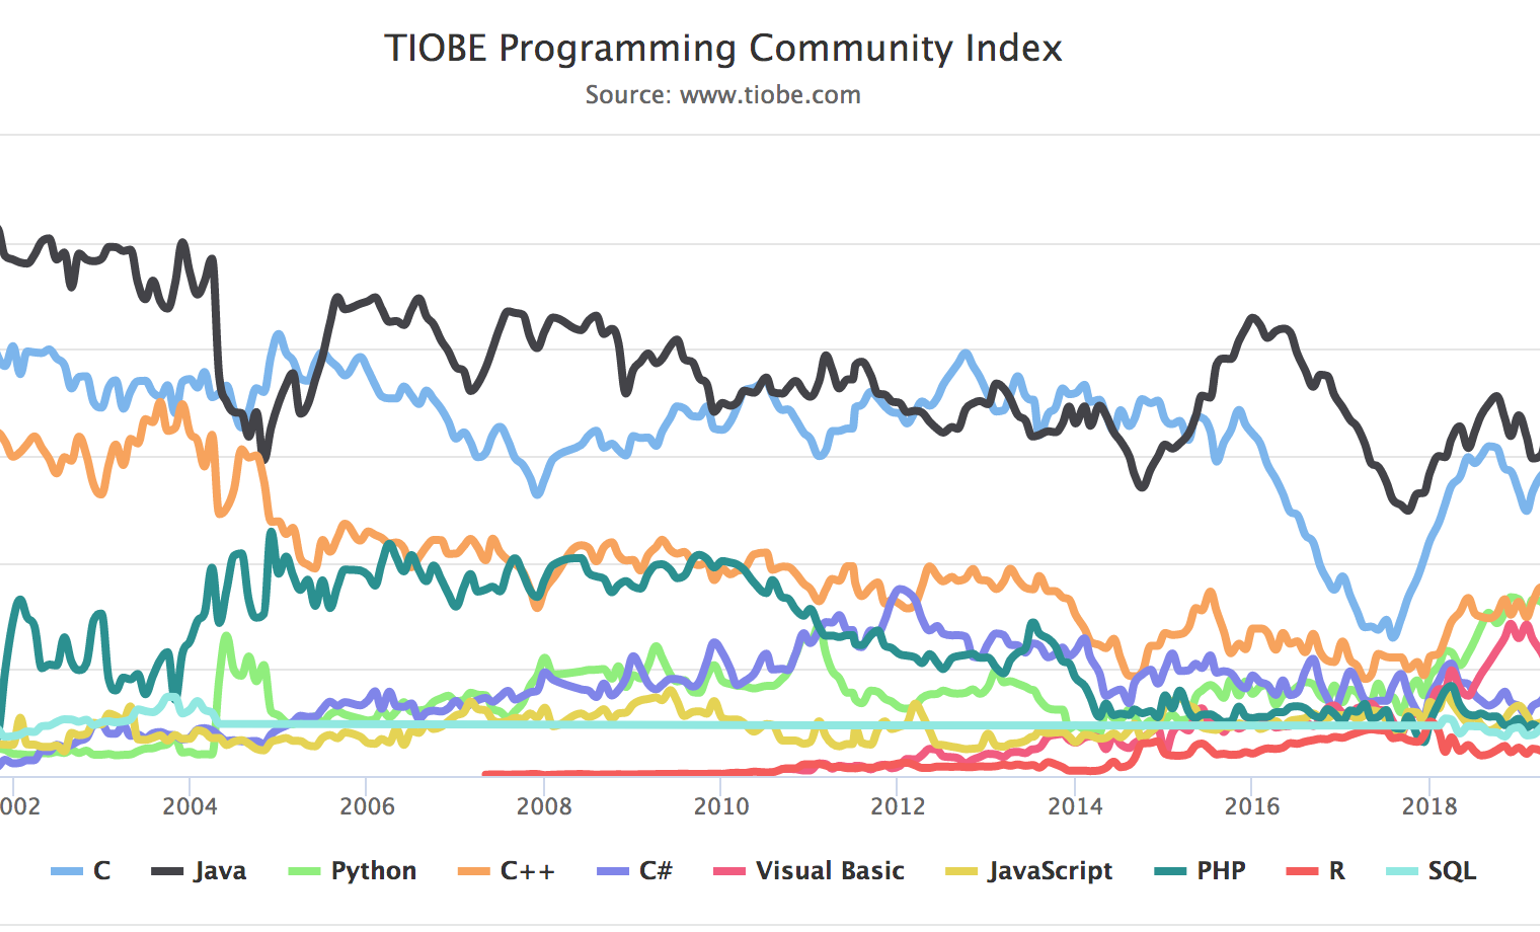
\includegraphics[width=0.95\textwidth]{assets/images/tiobe-index-1.png}
%         \caption{Indice di popolarità del \cplusplus}
%     \end{figure}
% \end{frame}

% \begin{frame}{Popolarità del \cplusplus}
%     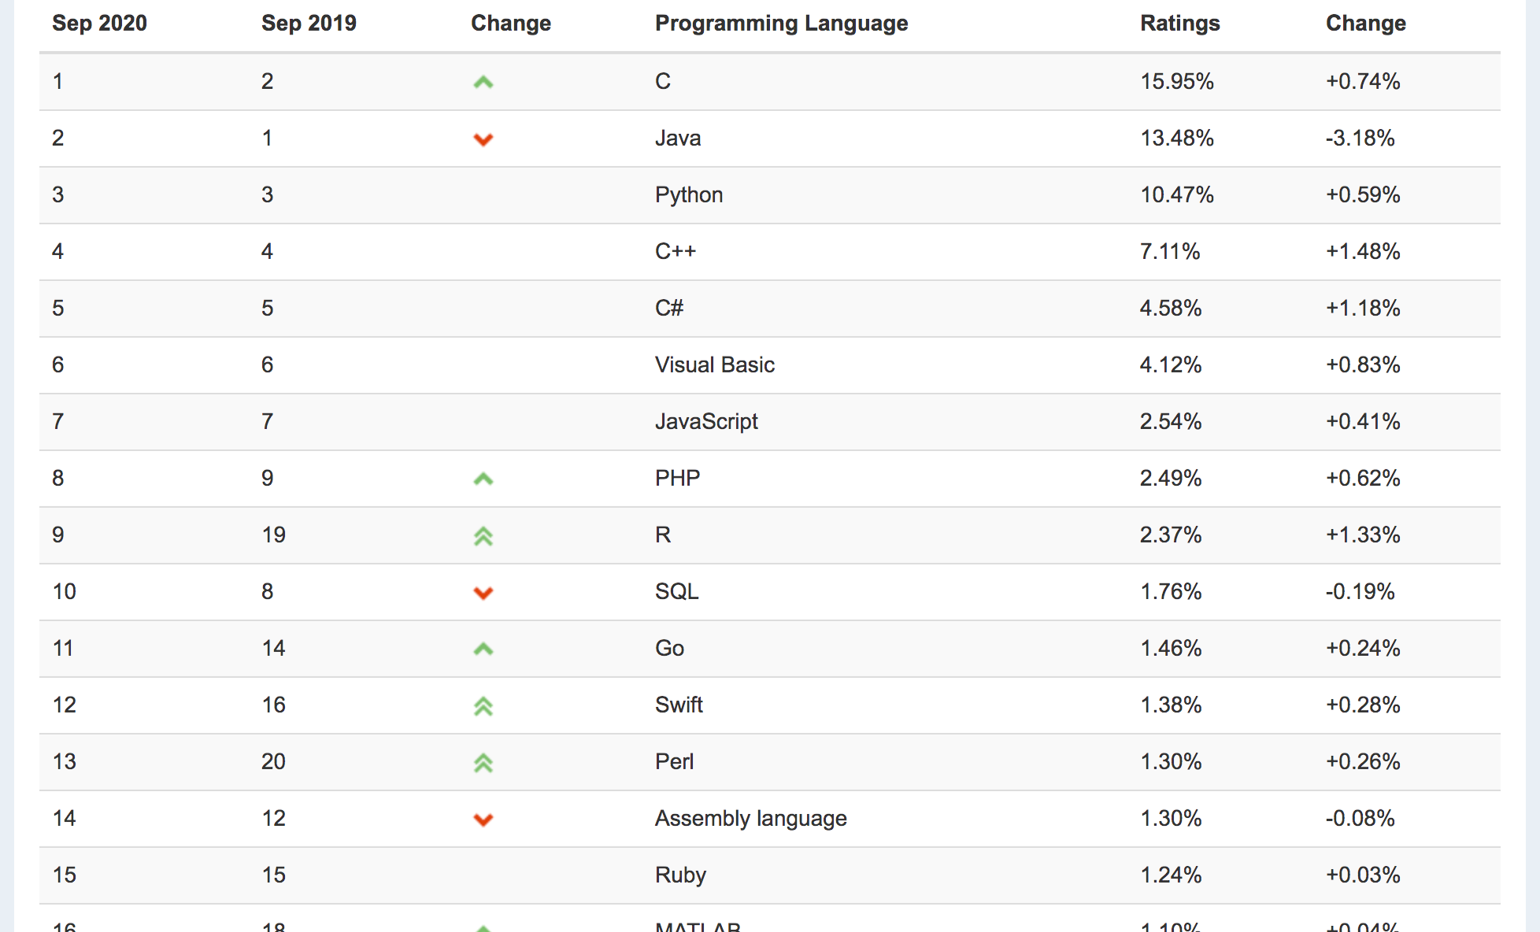
\includegraphics[width=0.95\textwidth]{assets/images/tiobe-index-2.png}
% \end{frame}

% \subsection{\cplusplus evoluzione}

\begin{frame}{Frame Title}
    \begin{itemize}[<+- | alert@+>]
        \item Comunità di utilizzatori
        \item Attori di peso (Microsoft, Google\dots)
        \item Standardizzazione
        \item Opinione: si evolve come un linguaggio naturale
    \end{itemize}
\end{frame}

\subsection{Applicazioni}

\subsection{Principi di progetto del \cplusplus}

\section{Copia profonda in \cplusplus}

\begin{frame}[fragile]{Frame Title}
            \begin{minted}[mathescape,
                tabsize=4,
                fontsize=\scriptsize,
                framesep=2mm]{cpp}
#include <string> // importazione librerie
#include <iostream>

using namespace std; // definizione spazio dei nomi

#ifndef CLASSE_B // guardi di compilazione
#define CLASSE_B

class B {
      string s;
public:
      B(string _s); // costruttore
      string get_s(); // getter
};

#endif
            \end{minted}
\end{frame}

\end{document}
